\documentclass{standalone}
\usepackage{tikz}
\usetikzlibrary{patterns, positioning}
\usepackage[sfdefault]{ClearSans} %% option 'sfdefault' activates Clear Sans as the default text font
\usepackage[T1]{fontenc}

\begin{document}
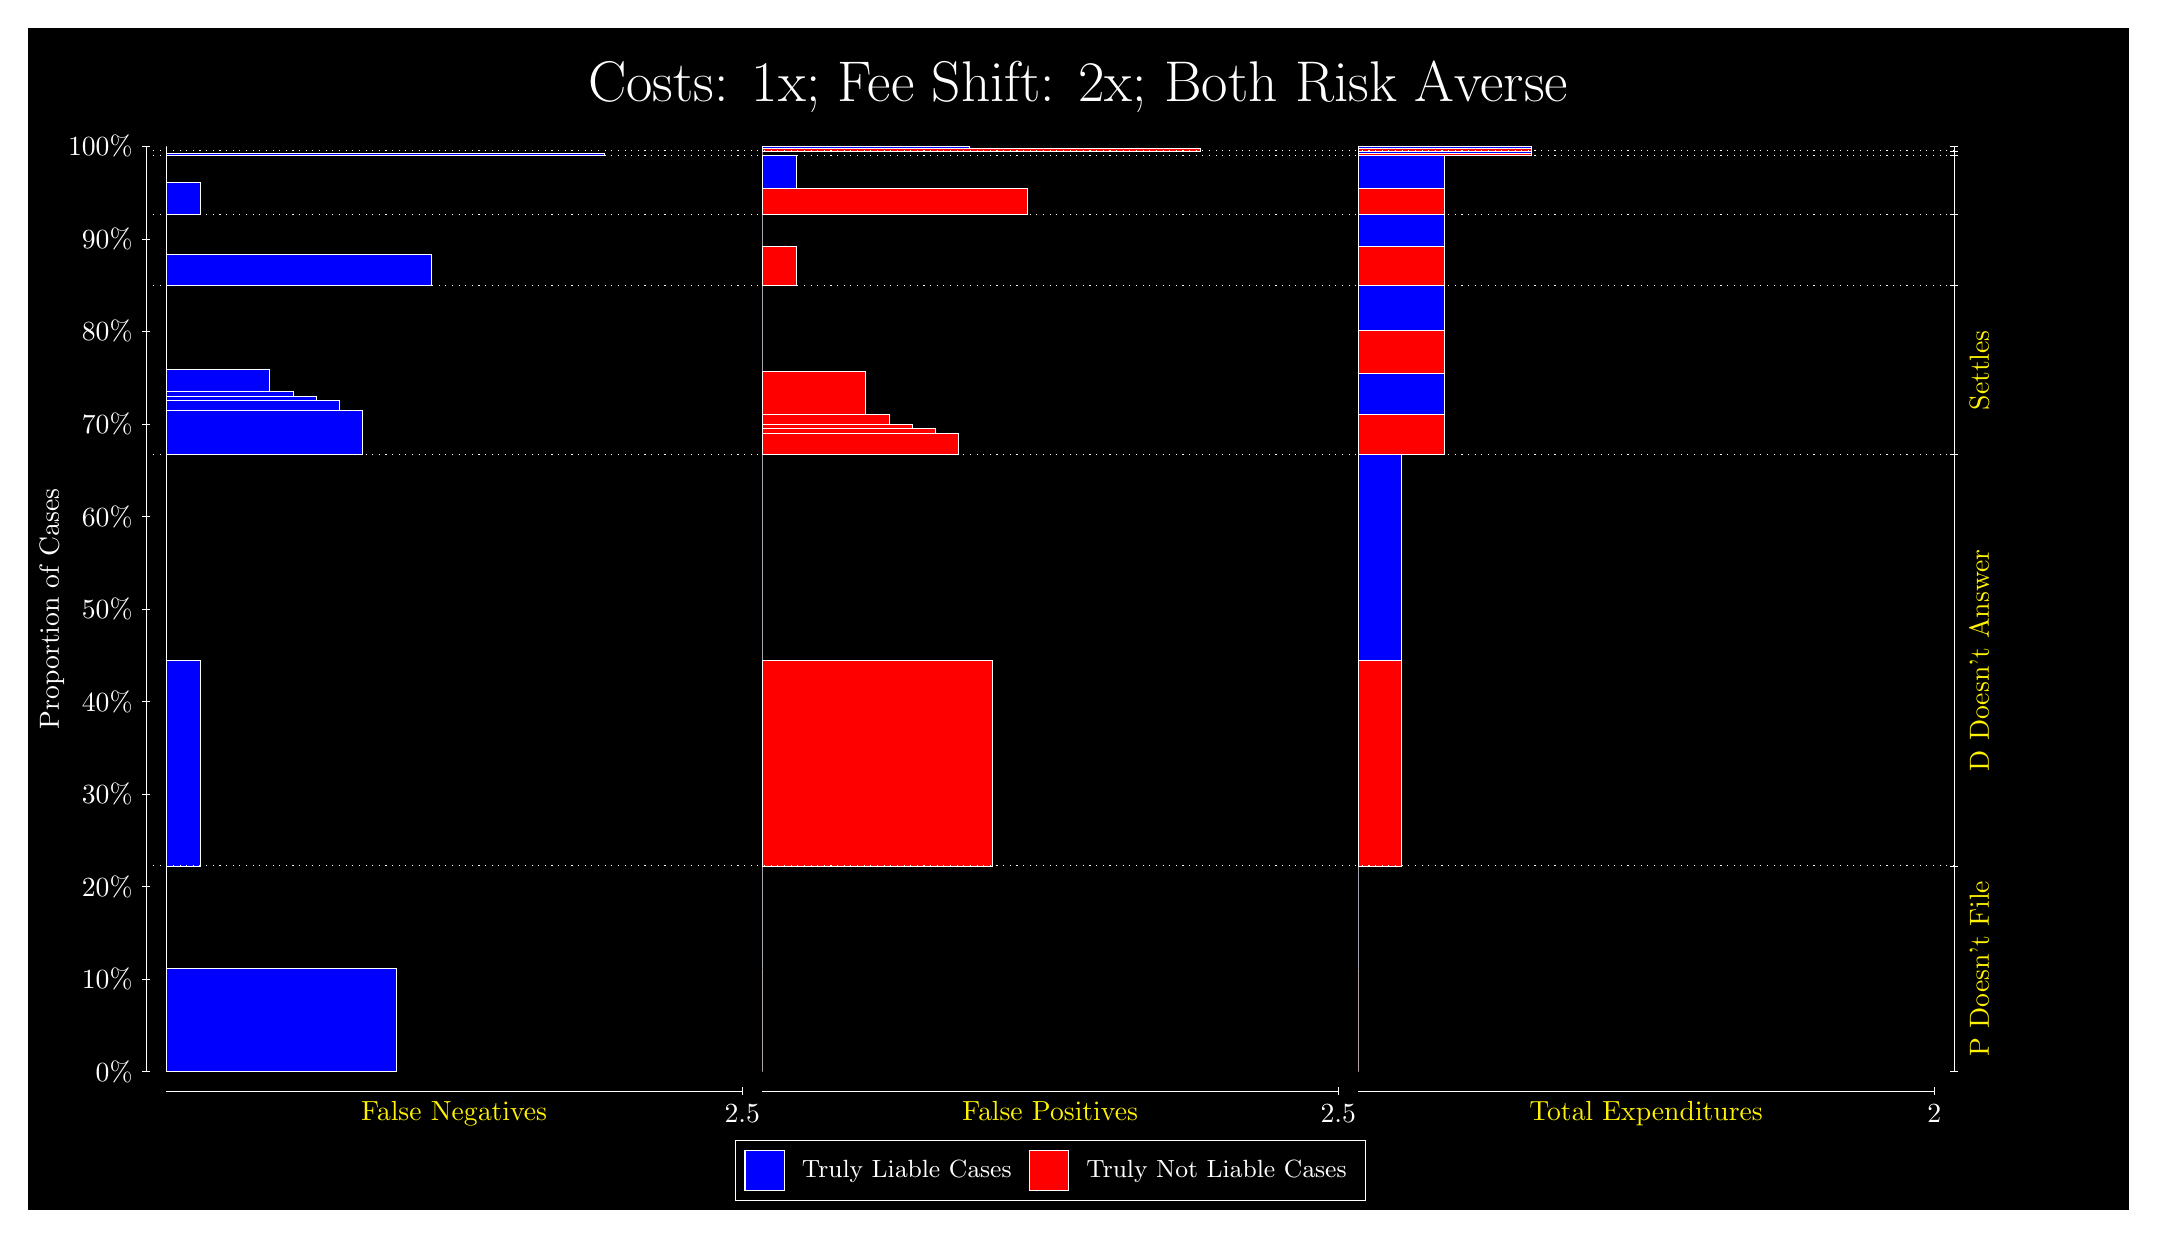
\begin{tikzpicture}
\draw[fill=black] (0,0) rectangle (26.667,15);
\draw[text=white] (0,13.5) rectangle (26.667,15) node[midway] {\huge Costs: 1x; Fee Shift: 2x; Both Risk Averse};
\draw[white, very thin] (1.5,1.75) -- (1.5,13.5);
\node[rotate=90, text=white, anchor=center] at (0.3, 7.625) {Proportion of Cases};
\draw[white, very thin] (1.45,1.75) -- (1.55,1.75);
\node[text=white, anchor=east] at (1.45, 1.75) {0\%};
\draw[white, very thin] (1.45,2.925) -- (1.55,2.925);
\node[text=white, anchor=east] at (1.45, 2.925) {10\%};
\draw[white, very thin] (1.45,4.1) -- (1.55,4.1);
\node[text=white, anchor=east] at (1.45, 4.1) {20\%};
\draw[white, very thin] (1.45,5.275) -- (1.55,5.275);
\node[text=white, anchor=east] at (1.45, 5.275) {30\%};
\draw[white, very thin] (1.45,6.45) -- (1.55,6.45);
\node[text=white, anchor=east] at (1.45, 6.45) {40\%};
\draw[white, very thin] (1.45,7.625) -- (1.55,7.625);
\node[text=white, anchor=east] at (1.45, 7.625) {50\%};
\draw[white, very thin] (1.45,8.8) -- (1.55,8.8);
\node[text=white, anchor=east] at (1.45, 8.8) {60\%};
\draw[white, very thin] (1.45,9.975) -- (1.55,9.975);
\node[text=white, anchor=east] at (1.45, 9.975) {70\%};
\draw[white, very thin] (1.45,11.15) -- (1.55,11.15);
\node[text=white, anchor=east] at (1.45, 11.15) {80\%};
\draw[white, very thin] (1.45,12.325) -- (1.55,12.325);
\node[text=white, anchor=east] at (1.45, 12.325) {90\%};
\draw[white, very thin] (1.45,13.5) -- (1.55,13.5);
\node[text=white, anchor=east] at (1.45, 13.5) {100\%};

\draw[white, very thin] (24.457,1.75) -- (24.457,13.5);
\draw[white, very thin] (24.407,1.75) -- (24.507,1.75);
\node[anchor=west] at (24.407, 1.75) {};
\draw[white, very thin] (24.407,4.3611) -- (24.507,4.3611);
\node[anchor=west] at (24.407, 4.3611) {};
\draw[white, very thin] (24.407,9.5833) -- (24.507,9.5833);
\node[anchor=west] at (24.407, 9.5833) {};
\draw[white, very thin] (24.407,11.729) -- (24.507,11.729);
\node[anchor=west] at (24.407, 11.729) {};
\draw[white, very thin] (24.407,12.636) -- (24.507,12.636);
\node[anchor=west] at (24.407, 12.636) {};
\draw[white, very thin] (24.407,13.385) -- (24.507,13.385);
\node[anchor=west] at (24.407, 13.385) {};
\draw[white, very thin] (24.407,13.442) -- (24.507,13.442);
\node[anchor=west] at (24.407, 13.442) {};
\draw[white, very thin] (24.407,13.5) -- (24.507,13.5);
\node[anchor=west] at (24.407, 13.5) {};

\draw[white, very thin, fill=blue] (1.75,1.75) rectangle (4.6775,3.0556);
\draw[white, very thin, fill=red] (1.75,3.0556) rectangle (1.75,4.3611);
\draw[white, very thin, fill=blue] (1.75,4.3611) rectangle (2.1891,6.9722);
\draw[white, very thin, fill=red] (1.75,6.9722) rectangle (1.75,9.5833);
\draw[white, very thin, fill=blue] (1.75,9.5833) rectangle (4.2384,10.151);
\draw[white, very thin, fill=blue] (1.75,10.151) rectangle (3.9457,10.278);
\draw[white, very thin, fill=blue] (1.75,10.278) rectangle (3.6529,10.326);
\draw[white, very thin, fill=blue] (1.75,10.326) rectangle (3.3602,10.383);
\draw[white, very thin, fill=blue] (1.75,10.383) rectangle (3.0674,10.67);
\draw[white, very thin, fill=red] (1.75,10.67) rectangle (1.75,11.729);
\draw[white, very thin, fill=blue] (1.75,11.729) rectangle (5.1167,12.131);
\draw[white, very thin, fill=red] (1.75,12.131) rectangle (1.75,12.636);
\draw[white, very thin, fill=blue] (1.75,12.636) rectangle (2.1891,13.048);
\draw[white, very thin, fill=red] (1.75,13.048) rectangle (1.75,13.385);
\draw[white, very thin, fill=blue] (1.75,13.385) rectangle (7.3123,13.411);
\draw[white, very thin, fill=red] (1.75,13.411) rectangle (1.75,13.442);
\draw[white, very thin, fill=red] (1.75,13.442) rectangle (1.75,13.469);
\draw[white, very thin, fill=blue] (1.75,13.469) rectangle (1.75,13.5);
\draw[white, very thin, fill=red] (9.3189,1.75) rectangle (9.3189,3.0556);
\draw[white, very thin, fill=blue] (9.3189,3.0556) rectangle (9.3189,4.3611);
\draw[white, very thin, fill=red] (9.3189,4.3611) rectangle (12.246,6.9722);
\draw[white, very thin, fill=blue] (9.3189,6.9722) rectangle (9.3189,9.5833);
\draw[white, very thin, fill=red] (9.3189,9.5833) rectangle (11.807,9.8528);
\draw[white, very thin, fill=red] (9.3189,9.8528) rectangle (11.515,9.9209);
\draw[white, very thin, fill=red] (9.3189,9.9209) rectangle (11.222,9.9756);
\draw[white, very thin, fill=red] (9.3189,9.9756) rectangle (10.929,10.098);
\draw[white, very thin, fill=red] (9.3189,10.098) rectangle (10.636,10.643);
\draw[white, very thin, fill=blue] (9.3189,10.643) rectangle (9.3189,11.729);
\draw[white, very thin, fill=red] (9.3189,11.729) rectangle (9.758,12.234);
\draw[white, very thin, fill=blue] (9.3189,12.234) rectangle (9.3189,12.636);
\draw[white, very thin, fill=red] (9.3189,12.636) rectangle (12.686,12.973);
\draw[white, very thin, fill=blue] (9.3189,12.973) rectangle (9.758,13.385);
\draw[white, very thin, fill=red] (9.3189,13.385) rectangle (9.3189,13.416);
\draw[white, very thin, fill=blue] (9.3189,13.416) rectangle (9.3189,13.442);
\draw[white, very thin, fill=red] (9.3189,13.442) rectangle (14.881,13.469);
\draw[white, very thin, fill=blue] (9.3189,13.469) rectangle (11.954,13.5);
\draw[white, very thin, fill=red] (16.888,1.75) rectangle (16.888,3.0556);
\draw[white, very thin, fill=blue] (16.888,3.0556) rectangle (16.888,4.3611);
\draw[white, very thin, fill=red] (16.888,4.3611) rectangle (17.437,6.9722);
\draw[white, very thin, fill=blue] (16.888,6.9722) rectangle (17.437,9.5833);
\draw[white, very thin, fill=red] (16.888,9.5833) rectangle (17.986,10.098);
\draw[white, very thin, fill=blue] (16.888,10.098) rectangle (17.986,10.617);
\draw[white, very thin, fill=red] (16.888,10.617) rectangle (17.986,11.161);
\draw[white, very thin, fill=blue] (16.888,11.161) rectangle (17.986,11.729);
\draw[white, very thin, fill=red] (16.888,11.729) rectangle (17.986,12.234);
\draw[white, very thin, fill=blue] (16.888,12.234) rectangle (17.986,12.636);
\draw[white, very thin, fill=red] (16.888,12.636) rectangle (17.986,12.973);
\draw[white, very thin, fill=blue] (16.888,12.973) rectangle (17.986,13.385);
\draw[white, very thin, fill=red] (16.888,13.385) rectangle (19.083,13.416);
\draw[white, very thin, fill=blue] (16.888,13.416) rectangle (19.083,13.442);
\draw[white, very thin, fill=red] (16.888,13.442) rectangle (19.083,13.469);
\draw[white, very thin, fill=blue] (16.888,13.469) rectangle (19.083,13.5);
\draw[white, dotted] (1.5,4.3611) -- (24.457,4.3611);
\draw[white, dotted] (1.5,9.5833) -- (24.457,9.5833);
\draw[white, dotted] (1.5,11.729) -- (24.457,11.729);
\draw[white, dotted] (1.5,12.636) -- (24.457,12.636);
\draw[white, dotted] (1.5,13.385) -- (24.457,13.385);
\draw[white, dotted] (1.5,13.442) -- (24.457,13.442);
\draw[white, very thin] (1.75,1.5) -- (9.0689,1.5);
\node[text=yellow, anchor=north] at (5.4094, 1.5) {False Negatives};
\draw[white, very thin] (9.0689,1.45) -- (9.0689,1.55);
\node[text=white, anchor=north] at (9.0689, 1.45) {2.5};

\draw[white, very thin] (9.3189,1.5) -- (16.638,1.5);
\node[text=yellow, anchor=north] at (12.978, 1.5) {False Positives};
\draw[white, very thin] (16.638,1.45) -- (16.638,1.55);
\node[text=white, anchor=north] at (16.638, 1.45) {2.5};

\draw[white, very thin] (16.888,1.5) -- (24.207,1.5);
\node[text=yellow, anchor=north] at (20.547, 1.5) {Total Expenditures};
\draw[white, very thin] (24.207,1.45) -- (24.207,1.55);
\node[text=white, anchor=north] at (24.207, 1.45) {2};

\node[text=yellow, centered, rotate=90] at (24.777, 3.0556) {P Doesn't File};
\node[text=yellow, centered, rotate=90] at (24.777, 6.9722) {D Doesn't Answer};
\node[text=yellow, centered, rotate=90] at (24.777, 10.656) {Settles};





\draw (12.978300999999998,1.5) node[draw=none] (baseCoordinate) {};
\begin{scope}[align=center]
        \matrix[scale=0.5, draw=white, below=0.5cm of baseCoordinate, nodes={draw}, column sep=0.1cm]{
            \node[rectangle, draw, minimum width=0.5cm, minimum height=0.5cm, fill=blue] {}; &
            \node[draw=none, font=\small, text=white] (B) {Truly Liable Cases}; &
            \node[rectangle, draw, minimum width=0.5cm, minimum height=0.5cm, fill=red] {}; &
            \node[draw=none, font=\small, text=white] (B) {Truly Not Liable Cases}; \\
            };
\end{scope}

\end{tikzpicture}
\end{document}